\documentclass[lettersize,journal]{IEEEtran}
\usepackage{amsmath,amsfonts}
\usepackage{algorithmic}
\usepackage{algorithm}
\usepackage{array}
\usepackage[caption=false,font=normalsize,labelfont=sf,textfont=sf]{subfig}
\usepackage{textcomp}
\usepackage{stfloats}
\usepackage{url}
\usepackage{verbatim}
\usepackage{graphicx}
\usepackage{cite}
\hyphenation{op-tical net-works semi-conduc-tor IEEE-Xplore}
\usepackage{booktabs}
\usepackage{amsmath,amsfonts}
\usepackage{algorithmic}
\usepackage{array}
\usepackage{textcomp}
\usepackage{stfloats}
\usepackage{subcaption}
\usepackage{url}
\usepackage{verbatim}
\usepackage{graphicx}
\usepackage{float}
\usepackage{titlesec}
\usepackage{amsthm}
\usepackage{mathtools}
\usepackage{gensymb}
\usepackage{hyperref}
\usepackage{amssymb}
\usepackage{amsmath}
\usepackage{dsfont}


\newcommand{\rEarth}{R_{\oplus}}
\newcommand{\viiva}{\mathop{\Bigg/}}
\newcommand{\sij}[3]{\viiva\limits_{\hspace*{-5mm}{#1}}^{\hspace*{5mm}{#2}}{#3}}
\newcommand{\R}{\mathbb{R}}
\newcommand{\N}{\mathbb{N}}
\newcommand{\B}[1]{\mathbf{#1}}
\newtheorem{theorem}{Theorem}
\newtheorem{corollary}{Corollary}
\newtheorem{lemma}[theorem]{Lemma}
\newtheorem{prop}[theorem]{Proposition}
\newtheorem*{remark}{Remark}

\def\BibTeX{{\rm B\kern-.05em{\sc i\kern-.025em b}\kern-.08em
    T\kern-.1667em\lower.7ex\hbox{E}\kern-.125emX}}
\begin{document}

\title{Stochastic geometry analysis of a narrow-beam LEO uplink with Gaussianmixture shadowing}
\author{IEEE Publication Technology,~\IEEEmembership{Staff,~IEEE,}
        % <-this % stops a space
\thanks{This paper was produced by the IEEE Publication Technology Group. They are in Piscataway, NJ.}% <-this % stops a space
\thanks{Manuscript received October 8, 2023; revised December 8, 2023.}}

% The paper headers
\markboth{Journal of \LaTeX\ Class Files,~Vol.~1, No.~2, December~2023}%
{Shell \MakeLowercase{\textit{et al.}}: A Sample Article Using IEEEtran.cls for IEEE Journals}

\IEEEpubid{}
% Remember, if you use this you must call \IEEEpubidadjcol in the second
% column for its text to clear the IEEEpubid mark.


\maketitle
\begin{abstract}
  This paper presents an in-depth analysis of the joint probability distributions of the Signal-to-Interference Ratio (SIR) and Signal-to-Interference-plus-Noise Ratio (SINR) in a narrow-beam Low Earth Orbit (LEO) satellite uplink system with interference cancellation techniques. The increasing deployment of LEO satellite constellations for global communication necessitates a thorough understanding of interference management and signal quality metrics to ensure reliable and efficient data transmission. We develop a comprehensive analytical framework to model the impact of narrow-beam antennas on both SIR and SINR, accounting for the critical factors influencing signal propagation and interference under LEO dynamics. Additionally, we explore various interference cancellation strategies to enhance system performance. By deriving closed-form expressions and conducting extensive simulations, we quantify the joint probabilities for different system parameters, providing valuable insights into the trade-offs and benefits of interference cancellation in these systems. Our findings offer practical guidelines for optimizing LEO uplink communication strategies, thereby contributing to the advancement of high-capacity and low-latency satellite communication networks. (CHAT GPT)
\end{abstract}

% Note that keywords are not normally used for peerreview papers.
\begin{IEEEkeywords}
  LEO, SIR meta distribution, Nakagami fading
\end{IEEEkeywords}


\section{Introduction}

In recent years, the deployment of Low Earth Orbit (LEO) satellite constellations has gained significant momentum due to their potential to provide global, high-speed, low-latency communication services. As the demand for such capabilities continues to rise, it becomes increasingly crucial to address the challenges associated with managing interference and maintaining robust signal quality within these systems. One of the primary metrics for assessing signal quality in communication systems is the Signal-to-Interference Ratio (SIR) and Signal-to-Interference-plus-Noise Ratio (SINR). These metrics become even more pertinent in LEO uplink scenarios, where multiple users concurrently transmit signals to satellites with limited frequency resources.

The narrow-beam antenna technology, which focuses transmission power into a smaller beamwidth, offers a promising approach to enhance signal quality and reduce interference. However, the dynamic nature of LEO satellites, coupled with the high density of ground terminals, creates complex interference scenarios that necessitate advanced analytical tools and methodologies for effective management. In this context, understanding the joint probability distributions of SIR and SINR becomes essential for designing robust LEO uplink systems.

This paper addresses this critical need by developing a comprehensive analytical framework to model the joint probability distributions of SIR and SINR in a narrow-beam LEO uplink environment. We incorporate various system parameters, such as satellite altitude, beamwidth, user density, and interference sources, to capture the intricate nature of signal propagation and interference in LEO systems. Furthermore, we investigate the effectiveness of different interference cancellation techniques, which are pivotal in mitigating interference and enhancing communication performance.

By deriving closed-form expressions and performing extensive simulations, our study provides valuable insights into the impact of narrow-beam antennas and interference cancellation on the joint probabilities of SIR and SINR. The results of this research not only shed light on the fundamental trade-offs and potential benefits of these technologies but also offer practical guidelines for optimizing LEO uplink communication strategies. Ultimately, this work aims to contribute to the advancement of high-capacity, reliable, and efficient satellite communication networks, paving the way for the continued growth and success of global connectivity solutions.





\begin{table}
  \begin{center}
    \begin{tabular}{| c | p{4.5cm}  |p{1.5cm}|}
      \hline
      \multicolumn{3}{|c|}{Glossary of principal symbols} \\
      \hline
      Symbol& Explanation &Value
      \\ 
      \hline
      $h$ & Altitude of the SBSs.&$1200$ [km] \\
      $\epsilon$ & Elevation angle of the SBSs.& $(90 \degree,40 \degree)$ \\
      $G[\cdot]$ & The SBS antenna gain.&\\
      $\alpha$ &Power path loss exponent.& $4$\\
      $\varphi_{\text{RX}}$ & Width of the SBSs $3$ dB gain.& $1.6 \degree$  \\
      $\Theta \subset E $ & Poisson p.p. on the earth's surface $E \subset \R^3$.& \\
      $\Phi \subset \R^2$ & Poisson p.p. on the plane. &\\
      $x_0$ & Nearest point to the origin in $\Phi$.&  \\
      $\lambda$ & Density parameter of $\Phi$ and $\Theta$.& \\
      $\kappa$ & Parameter that reflects the approximate mean number of UEs inside a SBS's $3$ dB footprint;  $\kappa = h^2\pi \lambda \varphi_{\textup{RX}}^2/\sin^4(\epsilon)$.& \\
      ${\tilde{\kappa}}$ &  $\kappa/\log(2)$.&\\
      $H_{\text{log}}$ & Log-normal shadowing mixture r.v.&     \\
      $p_{\text{LoS}}$& LoS probability & $(0.99,0.61)$\\
      $p_{\text{NLoS}}$&  $1-p_{\text{LoS}}$ & $(0.01,0.39)$\\
      $\mu_{\text{LoS}}$& Shadowing mean of the LoS component & 0 [dB] \\
      $\mu_{\text{NLoS}}$& Mean of the NLoS component & -26 [dB] \\
      $\sigma_{\text{LoS}}$& Variance of the LoS component & 4 [dB] \\
      $\sigma_{\text{NLoS}}$& Variance of the NLoS component & 6 [dB] \\
      $p_{\text{NLoS}}$&  $1-p_{\text{LoS}}$ & $(0.01,0.39)$\\
      $H_{\text{exp}}$ & Defective exponential shadowing r.v.    & \\
      $\theta$ & SIR or SINR threshold for a successful transmission.&\\
      $I$ & Interference at the typical SBS in the plane model.&\\
      $S$ & The signal power of the served UE at the typical SBS in the plane model.&\\
      $\mathring{I}$ & Interference at the typical SBS in the spherical model.&\\
      $\mathring{S}$ & The signal power of the served UE at the typical SBS in the spherical model.&\\ 
      $\hat{d}_{h,\epsilon}$ & The distance between the SBS and the center of the footprint in the plane model.&\\
      $d_{0}$ & Normalizing distance. & \\                        
      \hline
    \end{tabular}
  \end{center}
\end{table}   


\section{Quantities of interest}
\label{sec:analysissec}
We consider the ``typical SBS'' with a narrow Gaussian beam. The UEs are located on the plane according to the PPP. The SBS antenna boresigh is directed at $\textit{o} \in (0,0) \in \R^2$. The planar model approximates the spherical model, where the UEs are located on a spherical Earth's surface. We will come back to the spherical model in the numerical results section.



\subsection{Gain process}



The antenna gain loss depends on the distance $r$ from the origin $\textit{o} \in \mathbb{R}^2$ and is given by:

\begin{equation}
  G(r) = 2^{-r^2/\varphi_{\text{RX}}^2},
\end{equation}
where $\varphi_{\text{RX}}$ is the width of the $-3$ dB gain of an SBS, and $D_{h,\epsilon}$ is a scaling constant that depends on the altitude $h$ and elevation angle $\epsilon$ of the SBSs. The relevance of these parameters to the narrow-beam LEO satellite model is further discussed in Section \ref{sec:planarmodel}.

Given a homogeneous PPP $\Phi \subset \R^2$ of density $\lambda$ and i.i.d. fading variables $\{H_x\}_{x\in\Phi}$, we define the process of the perceived gains at the receiver; the gain process (GP):
\begin{equation}
  \label{eq:gainprocess}
  \mathcal{G} \triangleq \left\{ H_x G(D_{h,\epsilon}\|x\|):x \in \Phi  \right\}.
\end{equation}
The GP is a \textit{projection process} and, as such, a nonhomogeneous PPP [CITE]. The density of the GP has the following connection to the fading distribution.

Since the variables $\{H_x\}_{x \in \Phi}$ are i.i.d., we can denote the shadowing variable simply as $H$ without the subscript.


\begin{prop}[Density of the GP]
  Let $F_H(\cdot)$ be the complementary cdf (ccdf) of $H$. The density of $\mathcal{G}$ is given by
  \begin{equation}
    \label{eq:GPdensity}
    \lambda_{\mathcal{G}}(t)= \tilde{\kappa}F_H(t)/t, \text{ \text{for} }t>0,
  \end{equation}
  where $\tilde{\kappa}= \kappa/\log(2)$ and
  \begin{equation}
    \label{eq:kappa}
          {\kappa} \triangleq    \pi \lambda   \left(\frac{\varphi_{\textup{RX}}}{D_{h,\epsilon}}\right)^2.
  \end{equation}

  \begin{proof}
    Let $f_H(\cdot)$ be the pdf of $H$. We denote $G^{-1}(\cdot)$ as the generalized inverse $G^{-1}(y) = \inf \{x:G(x)<y\}$. By [CITE],
    \begin{align*}
      &\int_t^{\infty}\lambda_{\mathcal{G}}(y)dy \overset{}{=} \pi \lambda \mathbb{E}\left[ \left(\frac{G^{-1}(t/H)}{D_{h,\epsilon}}\right)^2 \right] \\
      &=\pi \lambda \int_t^{\infty} \left(-\frac{\varphi_{\text{RX}}\sqrt{-\log(t/h)}}{D_{h,\epsilon} \sqrt{\log(2)}}\right)^2f_H(h) dh  \\
      &= -\tilde{\kappa} \int_t^{\infty} \log(t/h)f_H(h) dh\\
      &\overset{(a)}{=} -\tilde{\kappa} \sij{t}{\infty} \log(t/h)F_H(h) - \tilde{\kappa} \int_t^{\infty}\frac{F_H(h)}{h} dh.
    \end{align*}
    In (a), we use the integration by parts. The result follows by differentiating w.r.t. $t$ and taking the negative sign. Note that a necessary condition for this operation is that $\int_t^{\infty} \log(t/h)f_H(h) \, dh$ converges for all $t > 0$.

  \end{proof}
\end{prop}

We will come back to the interpretation of the variable $\tilde{\kappa}$ in Section \ref{sec:numericalresultsandconnectiontoLEO}, where we explain the interpretation of the GP as approximate gains in a SBS in a LEO uplink with narrow-beamed SBSs.


We define the total interference, or the total received power, by
\begin{equation}
  \label{eq:totpow}
  I \triangleq \sum\limits_{x \in \Phi} H_x G(D_{h,\epsilon}\|x\|)=\sum\limits_{u \in \mathcal{G}}u.
\end{equation}
The symbol used to represent the points in the point process (p.p.) can be arbitrary. However, in \eqref{eq:totpow}, we use $u \in \mathcal{G}$ to avoid any potential confusion with $x \in \mathbb{R}^2$.

The mean and the variance of $I$ are given by
\begin{align}
  \label{eq:totmean}
  &\mathbb{E}\left(I \right) = \int_{0}^{\infty} t\lambda_{\mathcal{G}}(t) dt = \tilde{\kappa} \int_{0}^{\infty}F_H(t) dt \nonumber \\
  &=\tilde{\kappa} \mathbb{E}(H), \\\
  \label{eq:totvar}
  &\text{Var}\left(I \right) = \int_{0}^{\infty} t^2\lambda_{\mathcal{G}}(t) dt= \tilde{\kappa} \int_0^{\infty}tF_H(t) dt  \nonumber \\
  &= \tilde{\kappa} \frac{\text{Var}(H) + \mathbb{E}(H)^2}{2} = \tilde{\kappa}  \mathbb{E}[H^2]/2,
\end{align}
respectively.

The spatial path loss is of no interest in the definition of $I$ because we assume that the spatial path loss is a constant due to the narrow-beam antenna pattern decaying fast to $0$, $G(\cdot)$, which ensures that the relevant UEs are located near one another (see Section \ref{sec:numericalresultsandconnectiontoLEO}). Furthermore, given that the spatial path loss is identical for all transmitters, it does not influence the SIR. For the SINR, the noise variable can be scaled appropriately to account for the spatial path loss appropriately. Along these lines, we omit the spatial path loss between the SBS and UEs in $I$.






\subsection{Shadowing}
Unfortunately, unlike with a singular path loss, when the density of the projection process depends only on a single moment of $H$ regardless of its distribution, $\lambda_{\mathcal{G}}(t)$ has a pointwise dependence on $F_H(t)$. For analytical tractability, we use the defective exponential power fading distribution
\begin{equation}
  \label{eq:defexp}
  F_{{H}_{\text{Exp}}}(t)=\upsilon_{} e^{- t},
\end{equation}
 which is essentially an exponential mixture distribution, where $0 \leq 1-\upsilon_{} <1$ reflects the probability that the shadowed signal is blocked entirely and maps to $0$. We explain the correspondence of $\upsilon$ to the log-normal fading in Section \ref{sec:numericalresultsandconnectiontoLEO}.

         \begin{figure}[h]
           \centering
           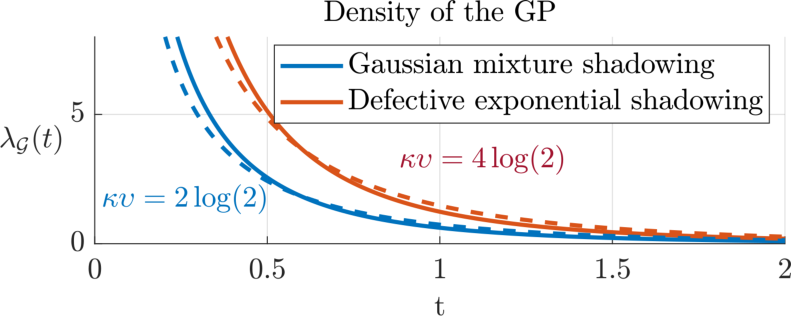
\includegraphics[width=\linewidth]{plotdensities.pdf}
           \caption{The density function of the GP for a two-tier log-normal mixure shadowing distribution with the corresponding exponential shadowing acquired by matching the first two moments. The parameters $\upsilon_{} \in \{0.85,0.53\}$ for the elevation angles $\epsilon \in \{90^{\circ},40^{\circ}\}$, respectively. The no-shadowing $H\equiv 1$ is also plotted for comparison.} 
           \label{fig:plotdensities}
         \end{figure}

%% \subsection{Slow-fading distribution}
%% While analytically tractable, the defective exponential distribution can capture the mean and the variance of a more complicated fading distribution with high variance, particularly the lognormal distribution, which is a well-established shadowing model in the LEO networks. The shadowing is defined by the mixed exponential RV
%% \begin{equation}
%%   \hat{H}_x \sim
%%   \begin{cases}
%%     0, \text{ if } U < 1-\rho,\\
%%     \text{Exp}(\mu), \text{ if } U \geq1- \rho,              \label{eq:tier2exponential}
%%   \end{cases}
%% \end{equation}
%% with $\mu>0$ and $0<\rho\leq1$, and $U \sim U(0,1)$ follows the uniform distribution.


%%where
%% \begin{align}
%%   &a=\frac{2 (p_{\text{LoS}}-1) e^{{\mu_{N\text{LoS}}}+\frac{{\sigma_{N\text{LoS}}}^2}{2}}-2 p_{\text{LoS}} e^{{\mu_{\text{LoS}}}+\frac{{\sigma_{\text{LoS}}}^2}{2}}}{(p_{\text{LoS}}-1) e^{2 \left({\mu_{N\text{LoS}}}+{\sigma_{N\text{LoS}}}^2\right)}-p_{\text{LoS}} e^{2 \left({\mu_{\text{LoS}}}+{\sigma_{\text{LoS}}}^2\right)}},\\
%%   &b=\frac{2 \left(({p_\text{LoS}}-1) e^{{\mu_{\text{N\text{LoS}}}}+\frac{{\sigma_{\text{N\text{LoS}}}}^2}{2}}-{p_\text{LoS}} e^{{\mu_{\text{LoS}}}+\frac{{\sigma_{\text{LoS}}}^2}{2}}\right)^2}{({p_\text{LoS}}-1) e^{2 \left({\mu_{\text{N\text{LoS}}}}+{\sigma_{\text{N\text{LoS}}}}^2\right)}-{p_\text{LoS}} e^{2 \left({\mu_{\text{LoS}}}+{\sigma_{\text{LoS}}}^2\right)}}.              
%% \end{align} 



\subsection{Laplace transform of the total received power}

With exponential shadowing ${H}_{\text{exp}}$, for Re$(s)>1$,

\begin{align}
  \label{eq:lapdef}
  &\mathcal{L}_{I}(s)\triangleq \mathbb{E}\left(e^{-sI}\right)= \exp\left\{-\int_0^{\infty}(1-e^{-sr}) \lambda_{\mathcal{G}}(r) dr \right\} \nonumber \\
  &=\exp\left\{-\tilde{\kappa}\int_0^{\infty}(1-e^{-sr}) F_{{H}_{\text{exp}}}(r) /r dr \right\} \nonumber \\
  &=\exp\left\{-\tilde{\kappa}\upsilon_{}\int_0^{\infty}(1-e^{-sr}) e^{-r} /r dr \right\} \nonumber \\
  &=(1+s)^{-\tilde{\kappa}\upsilon_{}},
\end{align}
which is the Laplace transform of the gamma distribution with the shape parameter $\tilde{\kappa}\upsilon_{}$. 


\subsection{SINR and STINR processes and their factorial moment measures}
Let $N \geq 0$ be the noise power constant. We denote the signal-to-interference-plus-noise ratio (SINR) process of the UEs as
\begin{align}
  \label{eq:SINR}
  \Psi &= \{\mathsf{Z}: \mathsf{Z} \in \Psi\} \triangleq \left\{ \frac{u}{N+I-u} : u \in \mathcal{G}\right\} \nonumber \\
  &=\left\{ \frac{H_x G(D_{h,\epsilon}\|x\|)}{N+I-H_x G(D_{h,\epsilon}\|x\|)} : x \in \Phi\right\},
\end{align}
where $I$ is defined in \eqref{eq:totpow}. Similarly, the signal-to-total-interference-plus-noise (STINR) process is defined as
\begin{align}
  \label{eq:STINR}
  \Psi' &= \{\mathsf{Z}': \mathsf{Z}' \in \Psi'\} \triangleq \left\{ \frac{u}{N+I} : u \in \mathcal{G}\right\}.
\end{align}
We can always recover on process from another
\begin{equation}
  \Psi = \left\{ \frac{\mathsf{Z}'}{1- \mathsf{Z}'}: \mathsf{Z}' \in \Psi' \right\}, \hspace{0.3cm} \Psi' = \left\{ \frac{\mathsf{Z}}{1+ \mathsf{Z}}: \mathsf{Z} \in \Psi \right\}.
\end{equation}
Let $\theta$ denote the SINR threshold of successful transmission. The event $\Psi \ni\mathsf{Z}> \theta$ is equivalent to $\Psi' \ni \mathsf{Z}'> \theta'$  with $\theta' \triangleq \theta/(1+\theta)$ and $\theta \triangleq \theta'/(1-\theta')$.

The factorial moment measure of the SINR process is defined on the sets $(t_1,\infty] \times \dots \times (t_n, \infty]$ with $t_1,\dots,t_n\geq 0$
    \begin{align}
      &M^{(n)}(t_1,\dots,t_n) \triangleq M^{(n)}((t_1,\infty],\dots,(t_n,\infty]) \nonumber \\
          & \triangleq \mathbb{E} \left( \sum^{\text{distinct}}_{\left(\mathsf{Z}_1, \dots, \mathsf{Z}_n \right) \in (\Psi)^{\times n}} \prod_{i=1}^n \mathds{1}(\mathsf{Z}_i >t_i)\right),
    \end{align}
    where $\mathds{1}(\cdot)$ is the indicator function, and ``distinct'' indicates that $\mathsf{Z}_i \neq \mathsf{Z}_j $ for all $i \neq j $. Similarly, for the STINR process,
    \begin{align}
          &M'^{(n)}(t'_1,\dots,t'_n) \triangleq M'^{(n)}((t'_1,\infty],\dots,(t'_n,\infty]) \nonumber \\
              &\triangleq \mathbb{E} \left( \sum^{\text{distinct}}_{\left(\mathsf{Z}'_1, \dots, \mathsf{Z}'_n \right) \in (\Psi')^{\times n}} \prod_{i=1}^n \mathds{1}(\mathsf{Z}'_i >t'_i)\right).
    \end{align}
 The (partial) density of the factorial moment measure of the STINR process is given by the successive partial differentiation of $M'^{(n)}$:
    \begin{align}
      \label{eq:differatemomentmeasure}
     &{\mu'}_n^{(n+i)}(z'_1,\dots,z'_n,\overbrace{z'_n,\dots,z'_n}^{\#i}) \nonumber \\&= (-1)^n \frac{\partial^n M'^{(n)}(t'_1\dots t_n',z'_n \dots z'_n) }{\partial t'_1 \dots \partial t'_n} |(t'_1=z_1'\dots t'_n=z'_n),
    \end{align}
    for $\sum_{i=1}^n z'_i + i z'_n\leq 1$ and $0$ otherwise.  If $i >0$, $\eqref{eq:differatemomentmeasure}$ is the \textit{partial density} of the $n$th factorial moment measure.

    The density of the $n$th factorial moment measure of the SINR process can be extracted from $\mu'^{(n)}$:
    \begin{align}
      \label{eq:densitySINR}
      &\mu^{(n)}(z_1,\dots,z_n) \nonumber\\
      &= \prod_{j=1}^n\frac{1}{(1+z_j)^2}\mu'^{(n)}\left(\frac{z_1}{1+z_1},\dots,\frac{z_n}{1+z_n}\right).
    \end{align}

    
  
\subsection{Order statistics of the STINR process}
We denote $\mathsf{Z}'_{(1)}>\mathsf{Z}'_{(2)} >\mathsf{Z}'_{(3)} \dots$ the order statistics of the STINR process $\Psi'$, such that $\mathsf{Z}'_{(1)}$ is the larges value in $\Psi'$.


The joint pdf $k$ strongest values of the STIR process $(\mathsf{Z}'_{(1)}, \dots, \mathsf{Z}'_{(n)})$ is given as a series expansion involving the partial densities
\begin{equation}
  \label{eq:jointprobability}
  f'_{(k)}(z'_1,\dots,z'_k)= \sum^{i_{\text{max}}}_{i=0}\frac{(-1)^i}{i!}{\mu'}_k^{(k+i)}(z'_1,\dots,z'_k),
\end{equation}
for $z'_1>z'_2>\dots>z'_k$ and $f'_{(k)}(z'_1,\dots,z'_k) =0 $ otherwise. The upper bound for the index $i_{\text{max}}<1/z'_k-k$ is the non-zero terms of the series expansion. 

The $k$-coverage probability that the first $k$ strongest signals reach the threshold $\theta$ is given by
\begin{align}
  \label{eq:kprobability}
  &\mathcal{P}^{(k)}(\theta) \triangleq  \int_{\theta'}^1\dots \int_{\theta'}^1 f'_{(k)}({z'_1},\dots,{z'_k})dz'_1 \dots d{z'_k}, \nonumber\\
  &=\sum_{i=0}^{i_{\text{max}}}\frac{(-1)^i}{i!}\int_{\theta'}^1\dots \int_{\theta'}^1 {\mu'}_k^{(k+i)}(z'_1,\dots,z'_k) \nonumber\\
  &\hspace{3.4cm}\times\mathds{1}(z'_1>\dots>z'_k) dz'_1 \dots d{z'_k}
\end{align}
with $\theta'=\theta/(1+\theta)$ and $i_{\text{max}}<1/\theta'-k$.

We still need to explicitly determine the expressions for the partial density ${\mu'}_n^{(n+i)}$ of the factorial moment measure $M^{(n)}$. We will address this separately for the interference-limited (interference-only) channel and the interference-plus-noise-limited channel.


\subsection{Partial density of the factorial moment measure in the interference-limited channel}

\label{sec:partialdensitySIR}


In this section, we characterize $\mu_n'^{(n+i)}$ and the order statistics of the STIR process through the Poisson-Dirichlet distribution $\text{PD}(0, \upsilon_{})$. The Poisson-Dirichlet distributions have unique properties that we do not describe exhaustively here. A necessary condition for the distribution is that the descending sequence $(y_{(1)}, y_{(2)}, \dots)$ satisfies $\sum_{i=1}^{\infty} y_{(i)} = 1$. This condition holds for the STIR ($N=0$) process; see \eqref{eq:totpow} and \eqref{eq:STINR}. 



Let $(X_{t}, t \geq 0)$ be a \textit{gamma subordinator}, also known as the \textit{gamma process}. It is an increasing jump process that exhibits an infinite number of jumps within any given time interval. The increment of the process during a time interval follows a gamma distribution. This process is a special case of a Lévy process, characterized by the Lévy measure $\lambda(r) = {e^{-r}}/{r}$.

Let $(X_{t}, t \geq 0)$ be a \textit{gamma subordinator}, or the \textit{gamma process}. It is a increasing jump process with infinite jumps within each time interval. The increments within each time interval are gamma distributed. It is a special case of the Lévy process characterized by the Lévy measure $\lambda(r) = e^{- r}/r$. Without a drift component, the Laplace transform of the gamma subordinator at time $t$ is given by
\begin{align}
  \label{eq:lapsubord}
  \mathbb{E}(\exp\{-s X_{t}\}) &= \exp\left\{-{t} \int_0^{\infty}(1-e^{-s r})\frac{e^{-r}}{r} dr \right\}. \nonumber \\
  &=(1+s)^{-t}.
\end{align}
But \eqref{eq:lapsubord} equals \eqref{eq:lapdef} at time $t=\tilde{\kappa}\upsilon_{} $. Hence, the total interference $I$ can be characterized by $X_{\tilde{\kappa} \upsilon_{}}$, which is again nothing but a gamma distributed r.v. of shape parameter $\tilde{\kappa}\upsilon_{}$. Let $V_1(X_{t}) \geq V_2(X_{t})\geq \dots \geq 0 $ denote the jumps of the gamma process at time $t$. We can formulate a random sequence
\begin{equation}
  \label{eq:relativesequence}
  \left(\frac{V_1(X_{\tilde{\kappa}\upsilon_{}})}{X_{\tilde{\kappa}\upsilon_{}}},\frac{V_2(X_{\tilde{\kappa}\upsilon_{}})}{X_{\tilde{\kappa}\upsilon_{}}} \dots \right).
\end{equation}
of normalized jumps of the subordinator. Directly from the definition, it is the STIR process $(\mathsf{Z}'_{(1)},\mathsf{Z}'_{(2)} \dots)$. It has the Poisson-Dirichlet distribution PD$(0, \upsilon_{} \tilde{\kappa})$. 




\begin{prop}
  The density of the n\textit{th} factorial moment measure of the STIR process at the narrow-beam LEO with the Gaussian antenna beam is given by
  \begin{align}
    \label{eq:factorialmoment}
    \mu'^{(n)}(t_1',\dots,t'_n) = (\tilde{\kappa}\upsilon_{})^n\prod_{j=1}^n{t'}_{j}^{-1}\left(1- \sum_{j=1}^nt'_j \right)^{\tilde{\kappa}\upsilon_{}-1},       
  \end{align}
  whenever $t_1>\dots >t_n$ and $\sum_{i=1}^n t_i \leq 1$, and $0$ otherwise.
\end{prop}

The partial densities can be derived from the density of the $n$th factorial moment measure by integrating $\mu^{(n+i)}$ w.r.t. the last $i$ auxiliary variables (cf. \eqref{eq:differatemomentmeasure}).

\begin{align}
  \label{eq:auxillary}
  &{\mu'}_n^{(n+i)}(z'_1,\dots,z'_n) \nonumber \\
  &= \int_{z'_n}^1 \dots \int_{z'_n}^1 {\mu'}^{(n+i)}(z'_1,\dots,z'_n,\zeta'_1,\dots,\zeta'_i) d\zeta'_1 \dots d\zeta'_i,
\end{align}
the support of the density being in the region $\sum_{i=1}^nz'_i+iz'_n \leq 1$. 








\subsection{Partial density of the factorial moment measure in the interference-plus-noise-limited channel}


In the interference-plus-noise-limited channel, we derive the partial densities through differentiating the factorial moment measure.

\begin{prop}
  The $n$-moment measure of the STINR process is given by
  \begin{align}
    \label{eq:nthmomentmeasureSTINR}
      &M'^{(n)}(t'_1,\dots,t'_n) =\left(\tilde{\kappa} \upsilon_{}\right)^n \nonumber\\
      &\times \int_1^{\infty}\dots\int_1^{\infty} e^{-N\hat{T}_n\sum\limits_{i=1}^nt'_iv_i} \left(1+\hat{T}_n\sum\limits_{i=1}^nt'_iv_i\right)^{-\tilde{\kappa}\upsilon_{}} \nonumber\\
      &\times \frac{\prod\limits_{i=1}^nt'_i}{\sum\limits_{i=1}^nt'_iv_i}  \left[\sum\limits_{j=1}^n\frac{1}{\prod\limits_{i\neq j}\left(t'_i v_i+ t_i'\hat{T}_n\sum\limits_{k=1}^nt'_kv_k \right)} \right] dv_1 \dots dv_n,
    \end{align}
    where $\hat{T}_n= 1/(1-\sum_{i=1}^nt'_i)$.

    \begin{proof}
      The derivation is provided in Appendix \ref{app:factorialmomentmeasureoftheSTINR}.
    \end{proof}

\end{prop}
 


The partial densities $\mu_{n}'^{(n+i)}$ are obtained through the direct differentiation of $M'^{(n)}$, as shown in \eqref{eq:differatemomentmeasure}. While the differentiation of the integrand in \eqref{eq:nthmomentmeasureSTINR} is feasible and straightforward, it is a tedious task. This process can be performed using symbolic tools such as Mathematica. In this work, we omit the explicit representations of the differentiated integrands. The interference-only case can also be obtained in the manner presented in this section by setting $N=0$; however, the density given in Section \ref{sec:partialdensitySIR} is significantly less computationally intensive.


\subsection{SIR and SINR under interference cancellation}




Let $(u_{(1)}, \dots, u_{(k)}) \subset \mathcal{G}$ represent an ordered set of points in the GP, where $u_{(1)}$ denotes the strongest signal at the SBS. In the following, we consider the SINR of the $n$-th strongest signal, where $n \leq k$. The signals with indices in the set \\$n \ni \mathcal{K} \subset \{1, 2, \dots, k\}$ are canceled from the total interference. We denote the SINR under the interference cancellation (IC-SINR) as
\begin{equation}
  \label{eq:IC-SINR}
  \text{SINR}_{n,\mathcal{K}} \triangleq \frac{u_{(n)}}{N+I-\sum_{j \in \mathcal{K} } u_{(j)}}.
\end{equation}


The IC-SINR can be formulated in terms of the STINR process:

%% \begin{align}
%%   \label{eq:IC-SINRcond}
%%   \mathcal{P}_{\text{IC}}^{(n,k)}(\theta) &\triangleq \mathbb{P}\{\text{SINR}_{n,k} > \theta \} \nonumber \\
%%   &=\mathbb{P} \left\{ u_{(n)} >\theta\left(N+I-  \sum_{j=1}^ku_{(j)}\right)\right\} \nonumber\\
%%   &\overset{}{=}\mathbb{P} \left\{(1+\theta) \frac{u_{(n)}}{N+1}+ \theta \frac{\sum^{j\neq n}_{j\in\{1,\dots,k\}} u_{(j)}}{N+I}>\theta \right\} \nonumber \\
%%   &\overset{(a)}{=} \mathbb{P} \left\{ \mathsf{Z}'_{(n)}+\theta'\sum^{j\neq n}_{j\in\{1,\dots,k\}}\mathsf{Z}'_{(j)} +>\theta'\right\}.
%% \end{align}

\begin{align}
  \label{eq:IC-SINRcond}
   & \mathds{1}\{\text{SINR}_{n,\mathcal{K}} > \theta \} = \mathds{1} \left\{ u_{(n)} >\theta\left(N+I-  \sum_{j \in \mathcal{K}} u_{(j)}\right)\right\} \nonumber\\
  &\overset{}{=}\mathds{1} \left\{(1+\theta) \frac{u_{(n)}}{N+1}+ \theta \frac{\sum\limits^{}_{j\in \mathcal{K} \setminus \{n\}} u_{(j)}}{N+I}>\theta \right\} \nonumber \\
  &\overset{(a)}{=} \mathds{1} \left\{ \mathsf{Z}'_{(n)}+\theta'\sum^{}_{j\in \mathcal{K} \setminus \{n\}}\mathsf{Z}'_{(j)} +>\theta'\right\}.
\end{align}


In (a), we divide both sides by $(1+\theta)$, which leads to the final result by the equivalence $\theta' = \theta/(1+\theta)$. In the interference-limited channel, $\text{SIR}_{n,\mathcal{K}} \triangleq (\text{SINR}_{n,\mathcal{K}}|(N=0))$.




In independent interference cancellation (IIC), we cancel and decode all signals independently: if the first $k$ signals exceed the SINR threshold $\tau$, \textit{i.e.}, $\mathsf{Z}_{(j)} > \tau$ for all $j \in \{1,\dots,k\}$, we can subtract the $k$ strongest signals from the interference. An improvement for the IIC is the successive interference cancellation (SIC). First, we cancel and decode the strongest signal, then decode the second strongest signal by subtracting the strongest and second strongest signal from the interference, and so on. The SIC of the $k$ strongest signals requires a superposition of conditions
\begin{equation}
  \label{eq:SIC-SINRcond}
  \begin{cases}
    &\mathsf{Z}'_{(1)} > \tau'\\
    & \mathsf{Z}'_{(2)} + \tau' \mathsf{Z}'_{(1)}> \tau' \\
    &\hspace{1cm}\dots \\
    &\mathsf{Z}'_{(k)} + \tau' \sum_{j=1}^{k-1}\mathsf{Z}'_{(j)}> \tau'.
  \end{cases}
\end{equation}



Let us consider that the $n$th strongest signal is decoded directly if its SINR exceeds $\theta$; otherwise, signal cancellation is attempted. We denote the SINR with independent interference cancellation as \text{IIC-SINR}$_{n,k}$, where interference from signals with indices in the set $[k] \triangleq \{1, \dots, k\}$ is canceled if each $(\mathsf{Z}_{(1)}, \dots  \mathsf{Z}_{(k)})$, reaches the signal separation threshold $\tau$, for which the sufficient condition is only $\mathsf{Z}_{(k)}>\tau$. The coverage probability is defined by


\begin{equation}
  \label{eq:IIC-SINRprob}
  \mathcal{P}^{(n,k)}_{\text{IIC}}(\theta,\tau) \triangleq \mathbb{P}\begin{Bmatrix} \text{SINR}_{n,[k]}(\theta)>\theta & \text{if } \mathsf{Z}_{(k)}>\tau \\
\mathsf{Z}_{(n)}>\theta & \text{otherwise} \end{Bmatrix}.
\end{equation}
Similarly, under the SIC, SIC-SINR$_{n,k}$ coverage probability is defined by
\begin{align}
  \label{eq:SIC-SINRprob}
  &\mathcal{P}^{(n,k)}_{\text{SIC}}(\theta,\tau)  \nonumber\\
  &\triangleq \mathbb{P}\begin{Bmatrix} \text{SINR}_{n,[k]}(\theta)>\theta & \text{if for all }m\in\{1,\dots,k\}  \\
    & \mathsf{Z}'_{(m)}+\tau'\sum\limits_{j =1}^{m-1}\mathsf{Z}'_{(j)}>\tau'\\
\mathsf{Z}_{(n)}>\theta & \text{otherwise} \end{Bmatrix},
\end{align}
with $\tau'=\tau/(1+\tau)$.

We have that $\mathcal{P}^{(k)}_{\text{SIC}}(\theta,\tau)\geq \mathcal{P}^{(k)}_{\text{IIC}}(\theta,\tau) \geq \mathcal{P}^{(1)}(\theta)$ for all $0<\tau < \theta$. To quantify performance improvement, we examine the $1$-coverage probability, which is only the SINR without any IC, to SINR-IIC and SINR-SIC coverage probabilities..

\begin{align}
  \label{DeltSICIIC}
  \Delta^{(n,k)}_{\text{IIC}}(\theta,\tau) \triangleq \mathcal{P}^{(n,k)}_{\text{IIC}}(\theta,\tau)- \mathcal{P}^{(1)}(\theta),\nonumber\\
  \Delta^{(n,k)}_{\text{SIC}}(\theta,\tau) \triangleq \mathcal{P}^{(n,k)}_{\text{SIC}}(\theta,\tau)- \mathcal{P}^{(1)}(\theta),
\end{align}
where the $1$-coverage probability  $\mathcal{P}^{(1)}(\theta)$ is given in $\eqref{eq:kprobability}$. Using the joint pdf of the $k$th STIR order statistics \eqref{eq:jointprobability}, we have for the SIC-SINR
\begin{prop}
  \begin{align}
    \label{eq:SICprob}
    & \Delta^{(n,k)}_{\text{SIC}}(\theta,\tau) \nonumber\\
    &=\sum^{i_{\text{max}}}_{i=0} \int_{0}^{\theta'} \dots \int_{0}^{\theta'}\frac{(-1)^i}{i!}\prod_{m=1}^k\nonumber \\
    &\hspace{0.2cm}\times \mathds{1}\left( z'_m+ \tau'\sum_{j=1}^{m-1} z'_j>\tau' \right)  \mathds{1}\left(z'_n+  \theta'\sum_{j\in [k] \setminus \{n\}} z'_j>\theta' \right) \nonumber \\
    & \hspace{0.2cm}\times \mathds{1}(z'_1>\dots>z'_k){\mu'}_k^{(k+i)}(z'_1,\dots,z'_k) d z'_1 \dots d z'_k,
  \end{align}
  with the upper summation limit bounded by $i_{\text{max}} < 1/\tau'-1=1/\tau.$ 
  \begin{proof}
    The expression follows from the joint pdf of the order statistics \eqref{eq:jointprobability} by imposing the conditions \eqref{eq:IC-SINRcond} and \eqref{eq:SIC-SINRcond}. We have abbreviated the upper bound of $i_{\text{max}}$ to $1/\tau$ from the upper limit given in \eqref{eq:jointprobability}: $i_{\text{max}} < 1/z'_{k}-k‰$, and $i_{\text{max}} \rightarrow \infty$ as $z'_k \rightarrow 0$. Fortunately, the l.h.s. conditioning limits the support of the integrand for small $z'_k$. Namely, we have that $z'_{k}+\tau'\sum_{j=1}^{k-1}z'_{j}>\tau'$. By simple algebra, $\sum_{j=1}^{k-1}z_{j}> 1-z_{k}/\tau'$. Recall the condition on the non-zero terms of the density of $M'^{(k+i)}$:  $\sum_{j=1}^k z'_{j}+i z'_{k} =\sum_{j=1}^{k-1}z'_{j} +z'_{k}+i z'_{k}  \leq 1$. The condition certainly does \textit{not} hold if $1-z_{k}/\tau'+ z'_{k}+i z'_{n}>1$. We arrive at the inequality $z'_{k} \left(-1/\tau' + 1 +i \right)>0$. Divide both sides by $z'_{k}$, and the general upper bound of $i$ follows.




  \end{proof}
\end{prop}
The SINR-IIC$_{(k)}$ case $\Delta^{(k)}_{\text{IIC}}(\theta,\tau)$ can be obtained by dropping the summation term inside the LHS condition in $\eqref{eq:SICprob}$, essentially bounding the lower integration limit to $\tau'$.



\subsubsection{Density function of the SIR of the strongest signal}
Combining \eqref{eq:densitySINR}, \eqref{eq:jointprobability}, and \eqref{eq:factorialmoment}, we get a closed form for the SIR pdf of the strongest signal in the region $z\geq 1$:


\begin{equation}
  \label{eq:SIR1}
  f_{(1)}(z) = \frac {\tilde{\kappa}\upsilon_{}\left({z + 1} \right)^{-\tilde{\kappa}\upsilon_{}}} {z}.
\end{equation}




\begin{align}
  &\mathbb{E}(\text{SIR}_{1,\{1\}})  \geq\int_{1}^{\infty}f_{(1)}(z)zdz=\frac{\tilde{\kappa}\upsilon_{}2^{1-\tilde{\kappa}\upsilon_{} }}{\tilde{\kappa}\upsilon_{}-1}, \tilde{\kappa}\upsilon_{} >1, \\
  &\mathbb{E}(\text{SIR}^2_{1,\{1\}}) \geq \int_{1}^{\infty}f_{(1)}(z)z^2dz = \frac{(\tilde{\kappa}\upsilon_{}) ^2 2^{1-\tilde{\kappa}\upsilon_{} }}{(\tilde{\kappa}\upsilon_{} - 2)  (\tilde{\kappa}\upsilon_{} - 1)}, \nonumber\\
  &\hspace{6.5cm}\tilde{\kappa}\upsilon_{}>2 .
\end{align}
The mean and the second moment diverge for $\tilde{\kappa}b\leq 1$ and $\tilde{\kappa}b\leq 2$, respectively. This implies that the variance of the SIR of the strongest signal is undefined for $\tilde{\kappa}b \leq 1$ and infinite for $1 <\tilde{\kappa}b \leq 2$. The insight reflects that the user experience of the link quality varies significantly over the SBSs in the density region $\tilde{\kappa} \upsilon_{} \leq 2$. To achieve a consistent SBS performance, we have to make the network denser than what corresponds to $\tilde{\kappa} \upsilon_{} =2$. Recall $\eqref{eq:kappa}: \kappa = \tilde{\kappa}\log(2)$ reflects the average number of UEs inside a $3$ dB footprint of a SBS.  Additionally, the density is influenced by shadowing characteristics through the parameter  $0<\upsilon_{} \leq 1$. One way to improve user fairness is to through the IC, which can help maintain good average performance while reducing the variance in the SIR at the SBSs.

\subsubsection{Numerical results regarding the average and variance of the SIR without interference cancellation and using IIC and SIC}



For this section, recall the partial density $\mu_k^{k+1}$ of the STIR process \eqref{eq:auxillary} \eqref{eq:factorialmoment} and \eqref{eq:IIC-SINRprob}-\eqref{eq:SICprob}.

We observed that setting the signal detection threshold $\tau = -7$ \text{dB}, equivalent to $\tau = 10^{-7/10} \approx 0.2$, for the IIC and SIC, the respective values $k = 2$ and $k=3$ are good choices for the number of signals. We adopt these values as our baseline. In this section, we consider the SIR in of the strongest signal, \textit{i.e.}, $n=1$.

For the IIC, $k = 2$ generally gives the best improvement for the coverage probability. However, for the SIC, $k = 4$ can yield better results than $k = 3$, particularly for small $\theta$.  

It is crucial to note that using a smaller value of $\tau$ leads to different outcomes, typically increasing the optimal $k$. One challenge associated with the proposed mathematical expressions is that numerical computations become highly intensive as $\tau$ decreases and $k$ increases.


For $\upsilon_{} \tilde{\kappa}=2$, the expected SIR of the strongest signal without IC is given by
\begin{equation}
  \mathbb{E}(\text{SIR}_{1,\{1\}})= \int_{0}^{\infty}\mathcal{P}^{(1)}(y)dy \approx 1.4.
\end{equation}
 Recall, that the variance $\text{Var}(\text{SIR}_{1,\{1\}})=\infty$, which is not desirable of we want the users treated fairly, which would mean that each SBS would have a consistent SIR.

  By increasing $\upsilon_{} \tilde{\kappa}$ (modifying $\lambda,h,\epsilon$ or $\varphi_{\text{RX}}$), we can reduce the variance in the SIR while maintaining the performance. For example, $ \mathbb{E}$(IIC-SINR$_{2}) \approx \mathbb{E}(\text{SIC-SINR}_{3}) \approx 1.4$ for $\upsilon_{} \tilde{\kappa}\in \{2.6,3.8\}$, respectively. The IIC-SINR variance is calculated by
  $\text{Var}(\text{IIC-SINR}_{2})=\int_{0}^{\infty}y\mathcal{P}_{\text{IIC}}^{(2)}(y,\tau)dy -\left(\int_{0}^{\infty}\mathcal{P}_{\text{IIC}}^{(2)}(y,\tau)dy\right)^2  \approx 2.6$ Similarly, $\text{Var(SIC-SINR}_{3}) = 2\int_{0}^{\infty}y\mathcal{P}_{\text{SIC}}^{(3)}(y,\tau)dy-$ $\left(\int_{0}^{\infty}\mathcal{P}_{\text{SIC}}^{(3)}(y,\tau)dy\right)^2 \approx 2.9$. The standard deviation in both cases is below $2$, which is a remarkable improvement in the consistency of the link quality.



  Increasing $\tilde{\kappa}$ does not necessarily require more dense SBS constellation to ensure each UE ideally having a serving SBS. On the contrary, with interference cancellation, a single SBS might be able to serve multiple UEs with satisfactory SIR, especially when using SIC. In this work, we study this case for SIR-SIC.



  The integration of $\mathbb{E}(\text{SIC-SINR}_{3}),\text{Var}(\text{IIC-SINR}_{2})$, and $\text{Var(SIC-SINR}_{3})$ with the native tools of Mathemtiaca seems hopeless. Hence, the integration in the IIC and SIC were conducted by trapezoidal method by first evaluating the SINR-IIC and SINR-SIC the ccdf values (\textit{i.e.} coverage probabilities) pointwise for sufficiently many uniformly spaced $y$, and conducting the approximate integral with the trapezoidal method implemented into a module in Mathematica.  

  






\section{Numerical results and the connection to the satellite communications}

\label{sec:numericalresultsandconnectiontoLEO}
While the analysis presented in Section \ref{sec:analysissec} fundamentally relies on a planar homogeneous PPP model with Gaussian path loss and functions as a stochastic geometry network model with defective exponential fading, holding intrinsic mathematical interest independent of its specific interpretation as a LEO setting, in this section, we explicitly define the geometrical interpretation of our system model as a narrow-beam LEO uplink. Furthermore, we align the defective exponential fading with log-normal shadowing using parameters representative of an urban scenario. We represent numerical results for the order statistics of both the SIR and the SINR and compare various IC scenarios: SIR-IIC, SIR-SIC, SINR-IIC, and SINR-SIC.

Our findings indicate that employing IC significantly enhances the coverage probability. In a noise-limited channel with moderate noise, we demonstrate that the optimal value for the parameter $\tilde{\kappa} \upsilon_{}$ is approximately $\log(2)$, which maximizes the performance of the LEO uplink. Moreover, IC not only reduces the variance in both SIR and SINR (across a uniform distribution of SBSs) but also preserves overall performance. Thus, appropriate interference cancellation can improve user fairness in the network without compromising link quality.


\subsection{Gaussian mixture shadowing model}
\label{sec:guassianmixture}

Consider a two-tier Gaussian mixture fading model with the following parameters for the LoS and NLoS tiers, respectively: $\mu_{\text{LoS}} = 0$ dB, $\sigma_{\text{LoS}} = 4$ dB, $\mu_{\text{NLoS}} = -26$ dB, and $\sigma_{\text{NLoS}} = 6$ dB. Under this fading model, the i.i.d. shadowing r.v.'s of the transmitters follow a log-normal mixture distribution;
\begin{align}
  \label{eq:tier2lognormal}
  H_{\mathcal{M}\mathcal{L}\mathcal{N}} &\sim p_{\text{LoS}} \mathcal{L}\mathcal{N}(\rho \mu_{\text{LoS}}, (\rho \sigma_{\text{LoS}})^2) \nonumber \\
  &\quad + p_{\text{NLoS}} \mathcal{L}\mathcal{N}(\rho \mu_{\text{NLoS}}, (\rho \sigma_{\text{NLoS}})^2),
\end{align}
with $p_{\text{NLoS}} = 1 - p_{\text{LoS}}$. Considering the natural base of the log-normal distribution, the constant $\rho \triangleq \log(10)/10$ normalizes the parameters $\mu_{\text{LoS}}, \sigma_{\text{LoS}}, \mu_{\text{NLoS}},$ and $\sigma_{\text{NLoS}}$, ensuring that the r.v.'s, conditioned on the shadowing tiers and expressed in decibels of the power ratio, $10 \log_{10}(H_{\mathcal{MLN}}|\text{LoS})$ and $10 \log_{10}(H_{\mathcal{MLN}}|\text{NLoS})$, evaluate to Gaussian r.v.'s $\mathcal{N}(\mu_{\text{LoS}}, \sigma_{\text{LoS}}^2)$ and $\mathcal{N}(\mu_{\text{NLoS}}, \sigma_{\text{NLoS}}^2)$, respectively.



Recall the exponential shadowing distribution \eqref{eq:defexp} used in the analysis. We introduce a scaling term, $\Upsilon$, to ensure that the means of the log-normal mixture distribution and the defective exponential distribution match: $\mathbb{E}(\Upsilon H_{\mathcal{MLN}}) = \mathbb{E}(H_{\text{Exp}}) = \upsilon$. By equating the first two moments of $H_{\text{Exp}}$ (l.h.s.) and $\Upsilon_{} H_{\mathcal{M} \mathcal{L}\mathcal{N}}$ (r.h.s.)
\begin{equation}
  \label{eq:matchingmoments}
  \begin{cases}
    &\upsilon_{} = \Upsilon_{} \left(p_{\text{LoS}} e^{\mu_{\text{LoS}} + \sigma_{\text{LoS}}^2/2} + p_{\text{NLoS}} e^{\mu_{\text{NLoS}} + \sigma_{\text{NLoS}}^2/2}\right)\\
    &2\upsilon_{}= \Upsilon_{}^2 \left( p_{\text{LoS}} e^{2(\mu_{\text{LoS}} + \sigma_{\text{LoS}}^2)} + p_{\text{NLoS}} e^{2(\mu_{\text{NLoS}} + \sigma_{\text{NLoS}}^2)} \right), 
  \end{cases}
\end{equation}
 we can solve for the parameters
\begin{align}
  \label{eq:upsilon}
  & \upsilon_{}= \frac{ 2\left( p_{\text{LoS}}e^{\mu_{\text{LoS}}+\sigma^2_{\text{LoS}}/2}+p_{\text{NLoS}}e^{\mu_{\text{NLoS}}+\sigma^2_{\text{NLoS}}/2} \right)^2}{p_{\text{LoS}}e^{2(\mu_{\text{LoS}}+\sigma_{\text{LoS}}^2)}+p_{\text{NLoS}}e^{2(\mu_{\text{NLoS}}+\sigma_{\text{NLoS}}^2)}}, \\
    \label{eq:Upsilon}
    &\Upsilon_{} = \frac{2\left(p_{\text{LoS}}e^{\mu_{\text{LoS}}+\sigma^2_{\text{LoS}}/2}+p_{\text{NLoS}}e^{\mu_{\text{NLoS}}+\sigma^2_{\text{NLoS}}/2}\right)}{p_{\text{LoS}}e^{2(\mu_{\text{LoS}}+\sigma_{\text{LoS}}^2)}+p_{\text{NLoS}}e^{2(\mu_{\text{NLoS}}+\sigma_{\text{NLoS}}^2)}}.
\end{align}
Recall equations \eqref{eq:totmean} and \eqref{eq:totvar}. Matching the first two moments of any fading distributions is equivalent to matching the mean and variance of the total interference using the corresponding fading distributions.


Without loss of generality, we can set $\Upsilon = 1$ when studying SIR scenarios, as the scaling of the signal powers cancels out when $N = 0$. In the case of SINR, the scaling is accounted for by adjusting the noise constant by a factor of $N \sim 1/\Upsilon$. We will revisit this topic in the next section.

The parameter $0 \leq 1-\upsilon < 1$ of the defective exponential distribution encapsulates the occurrences of severe shadowing, where the signal is either blocked by an obstacle or destructively interfered by its multipath components to such an extent that the signal power approaches $-\infty$ dB in the Gaussian mixture shadowing model. Severe shadowing occurrences are particularly common at low elevation angles due to the presence of tall buildings and other large objects that prevent a clear line-of-sight (LoS), thus causing significant signal blockage.



\subsection{Interpretation as a planar model of a narrow-beam LEO uplink}
\label{sec:planarmodel}


As indicated in Section \ref{sec:analysissec}, we employ an infinite flat-earth model. This planar approximation effectively represents the spherical model described in Section \ref{eq:sphericalmodel}, particularly when considering the narrow Gaussian antenna beams $G(\cdot)$ at the SBSs. The UEs, acting as Earth transmitters, radiate omnidirectionally and are modeled as a homogeneous PPP $\Phi \subset \mathbb{R}^2$. The signals emitted by the UEs are subject to shadowing, which is modeled by i.i.d. exponential random variables $H_{\text{Exp}}$ with a non-zero probability measure at $0$, as described by the distribution function in \eqref{eq:defexp}. The SBS antenna boresight is directed towards the origin, denoted as $\textit{o} \triangleq (0,0)$. Figure \ref{fig:UEsontheplane} provides a geometric visualization of the planar LEO model.





Although the Gaussian function is an idealized antenna pattern, it accurately models the main lobe ($-10$ dB lobe) of several antenna patterns, for example, the ITU-R LEO reference radiation pattern, as shown in Figure \ref{fig:antennapats}.

\begin{figure}[h]
  \centering
  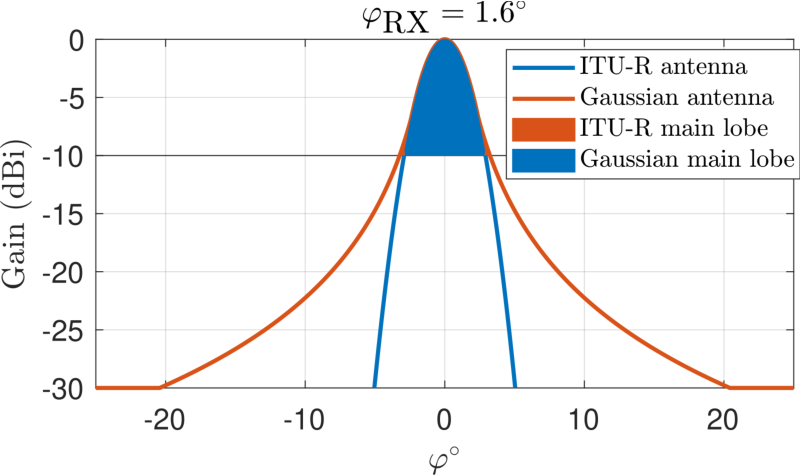
\includegraphics[width=\linewidth]{antennapats.pdf}
  \caption{Comparison between the Gaussian and \cite[ITU-R LEO reference radiation patterns]{ITURS1528}. The gain of the Gaussian antenna in the main lobe ($-10$ dB lobe) is almost identical to the ITU-R main lobe. However, there is a slight difference towards the edges of the main lobe. 
    %Sidelobes have significant differences. 
    The fast-decaying Gaussian beam essentially corresponds to the main lobe component.} 
  \label{fig:antennapats}
\end{figure}

Due to the ergodicity of the PPP, the model can be interpreted as a snapshot of a single realization of $\Phi$, with the averaging being performed over uniformly distributed SBSs rather than the ensemble of $\Phi$. For example, the coverage probabilities describe the fraction of SBSs that reach the threshold $\theta$.


The scaling term $D_{h,\epsilon} = {\sin^2(\epsilon)}/{h}$, where $\epsilon$ is the elevation angle of the satellite and $h$ is the altitude, that appears in the Gaussian antenna pattern path loss function $\|x\| \mapsto G(D_{h,\epsilon}\|x\|)$ in \eqref{eq:gainprocess}, is the first-order coefficient in the Taylor expansion of the function $\|x\| \mapsto \varphi_x$, where $\varphi_x$ is the angle between $x \in \Phi$ and the SBS in the planar model. In other words, $\varphi_x \approx D_{h,\epsilon}\|x\|$, which provides a tight approximation for narrow antenna beams. The derivation of this term is provided in Appendix \ref{app:constantD}.


The parameter $\kappa=\tilde{\kappa} \log(2)$ in the density function \eqref{eq:GPdensity} of $\mathcal{G}$ can be interpreted as the approximate average number of UEs within the $-3$ dB footprint of a SBS. This interpretation is derived by solving $D_{h,\epsilon}\|x_{\text{RX}}\| = \varphi_{\text{RX}}$ for the distance $\|x_{\text{RX}}\|$ to the edge of the $-3$ dB footprint, and then applying the area formula for a circle along with Campbell's theorem.


The constant $\tilde{\kappa} \upsilon_{}$, which encompasses the average number of UEs within a SBS $-3$ dB footprint $\kappa= \tilde{\kappa}\log(2)$, as well as the fraction of non-zero signals $\upsilon_{}$, appears as the only system parameter in the Laplace transform of $I$ \eqref{eq:lapdef} and the factorial moment measures of the STIR and STINR processes in \eqref{eq:factorialmoment} and \eqref{eq:nthmomentmeasureSTINR}, respectively. In other words, although $\tilde{\kappa}$ is connected to $h$, $\lambda$, $\varphi_{\text{RX}}$, and $\epsilon$, it is the sole spatial system parameter which independently determines the performance metrics alongside the shadowing-related parameter $\upsilon$.









As previously mentioned, we consider a narrow Gaussian antenna beam that rapidly decays to zero. Consequently, the relevant UEs are located in close proximity to one another. The spatial path loss law for \textit{all transmitters} is given by
\begin{equation}
  \label{eq:pathlosslaw}
  \ell(\hat{d}_{h,\epsilon}) \triangleq \left( {\hat{d}_{h,\epsilon}}/{d_0} \right)^{\alpha},
\end{equation}
where $\hat{d}_{h,\epsilon} \triangleq {h}/{\sin(\epsilon)}$ is the distance between the origin $\textit{o}$ and the SBS. The distance depends on the altitude $h$ and the elevation angle $\epsilon$ and can be derived using simple geometry, as illustrated in Figure \ref{fig:systemmodel}. The power path loss exponent $\alpha \geq 0$. Additionally, the normalizing distance $d_0$ accounts for other factors influencing the path loss, such as the frequency band of the signals, and ensures that the path loss is dimensionless.

Let $W\geq0$ be a dimensionless constant noise power at the SBS. Given that the conditions $$\frac{\Upsilon_{}u/\ell(\hat{d}_{h,\epsilon})}{\Upsilon_{}I/\ell(\hat{d}_{h,\epsilon}) + W}>\theta \text{ and } \frac{u}{I + W\ell(\hat{d}_{h,\epsilon})/\Upsilon_{}}> \theta,$$ for $u \in \mathcal{G}$, are equivalent, the spatial path loss can be incorporated into the noise term \begin{equation}N=W\ell(\hat{d}_{h,\epsilon})/\Upsilon_{}\end{equation} alongside the power scaling term $\Upsilon_{}$ introduced in Section \ref{sec:guassianmixture}---$N$ being introduced in \eqref{eq:SINR} and \eqref{eq:STINR} for the SINR and STINR processes, respectively. The constants $\ell(\hat{d}_{h,\epsilon})$ and $\Upsilon_{}$ are only relevant in the interference-plus-noise limited channel and can be disregarded for $W=N=0$.



\textbf{To summarize Sections \ref{sec:guassianmixture} and \ref{sec:planarmodel}:} Adjusting $N$ and $\upsilon$ are the only requirements to interpret the analysis in Section \ref{sec:analysissec} as a narrow Gaussian beam LEO setting with Gaussian mixture shadowing:

\begin{enumerate}
    \item Set the noise value $N = {W \ell(\hat{d}_{h,\epsilon})}/{\Upsilon}$, for a noise power at the SBS $W \geq 0$, according to \eqref{eq:Upsilon} and \eqref{eq:pathlosslaw}.
    \item Set $\upsilon \in (0,1]$ in $F_{\text{Exp}}(t) = \upsilon e^{-t}$ according to \eqref{eq:upsilon}.
\end{enumerate}


\begin{figure}[h]%
  \centering
  \subfloat[\centering  Interpretation of the \textit{planar} system model with the SBSs in adjacent orbits serving an urban area and a realization of the UEs. The altitudes are not to scale.]{{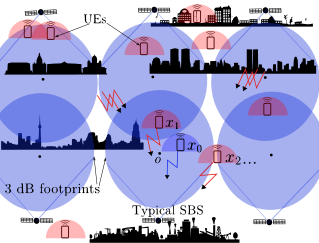
\includegraphics[width=\linewidth]{UEsontheplane.png}}
    \label{fig:UEsontheplane}%%
  } 
  \qquad
  \subfloat[\centering The typical SBS as seen from the side. The transmitters are projected into line $(0, \infty)$ according to their norm.]{{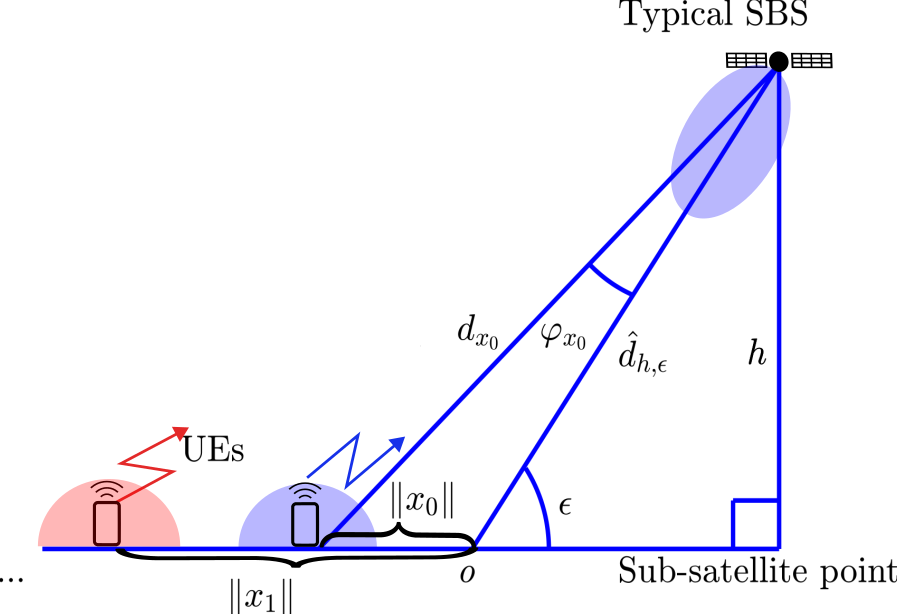
\includegraphics[width=\linewidth]{drawing.png}}     \label{fig:systemmodel}} %%
  \caption{The simplified narrow-beam LEO uplink system model. The SBS antenna boresight is oriented towards $\textit{o}$, the focus point of the elliptical footprint. The omnidirectionally transmitting UEs $\{x_i\}$ are located according to the HPPP on the plane. The nearest transmitter, $x_0$, is the served UE.}
\end{figure}







\subsection{Monte Carlso simulations of the spherical model}
\label{eq:sphericalmodel}
The base line system model is the spherical model, where the UE are located on the spherical Earths surface according to the PPP $\Theta$. Like in the planar model, the UEs are radiating omnidirectionally at power $P=1$ and are multiplied by i.i.d. random shadowing $H_x$.

The total received power at the typical SBS from the UEs in the PPP $\Theta \subset E \subset$ \textit{Earth surface} of density $\lambda$, with $E$ denoting the area above the horizon of the typical SBS (\textit{i.e.} the locations that are visible to the typical SBS) is defined as

\begin{equation}
  \label{eq:mathringptot}
  \mathring{I} \triangleq (\mathring{I}- \mathring{S}) + \mathring{S} =    \sum_{x \in \Theta} H_x\ell(d_x) = \sum_{x \in \Theta}  \frac{H_x G(\varphi_x)}{(d_x/d_0)^{\alpha}},
\end{equation}
where $H_{x} \sim H_{\mathcal{M}\mathcal{L}\mathcal{N}}$ are i.i.d. log-normal mixture r.v.'s inroduced in Section \ref{sec:guassianmixture}. The power path loss exponent $\alpha \geq 0$, and $(d_x/d_0)$ is the distance between the UE and the typical SBS, and the normalizing distance $d_0$ accounts for any other factors affecting the path loss, such as the frequency band of the signals, and casts the path loss to a dimensionless quantity. The sub-satellite point of the typical SBS is at $\textit{o}_E$. As with the planar model, $\varphi_x$ is the angle between the SBS antenna boresight and  $u \in \Theta$. However, in contrary to the planar model, this is calculated precicely the spherical model. $\mathring{S}$ is the strongest signal at the SBS and $\mathring{I}-\mathring{S}$ is the interference power from the other signals. The SIR and SINR $\mathring{S}/(\mathring{I}-\mathring{S})$,  $\mathring{S}/(\mathring{I}-\mathring{S}+N)$, are defined accordingly. The IC schemes SIR-IIC, SIR-SIC, SINR-IIC and SINR-SIC are simulated using these definitions through Monte Carlo simulations. 


The spherical model \eqref{eq:mathringptot} is unnesessarily complex to work analytically. However, for the narrow-beamed antenna gain, such as the Gaussian antenna beam, the planar model introduced in Section \ref{sec:planarmodel} stricingly well approximates the spherical model, like demonstratet in CITE LÄHDE. In this work, we exclude the practical implementation details of the spherical model Monte Carlo simulations and refer to [???] for an extensive comparison between the planar model and the spherical model in the narrow beam LEO upink. Also, the presented results derived from the analysis based in the planar model are always compared to the Monte Carlo simulations based in the spherical model formulated in this section.





%% \begin{verbatim}
%% \begin{table}
%% \begin{center}
%% \caption{Filter design equations  ...}
%% \label{tab1}
%%     \begin{tabular}{| c | c | c |c|}
%%       \hline
%%       & $\mathcal{P}^{(1)}(\cdot)$& $\mathcal{P}^{(2)}_{\text{IC}}(\cdot)$& $\mathcal{P}^{(2)}_{\text{SC}}(\cdot)$\\
%%       \hline
%%       $\mathbb{E}(\cdot)$&$1.4$ & $1.4$ &$1.4$\\ 
%%       \hline
%%       $\tilde{\kappa}$& $2/\upsilon_{} $ &$2.6/\upsilon_{}$& $3.4/\upsilon_{}$\\
%%       \hline
%%       Var$(\cdot)$& $\infty$ & $2.6$ &$2.3$\\
%%       \hline 
%%     \end{tabular}
%% \end{center}
%% \end{table}
%% \end{verbatim}


\appendices

\section{Factorial moment measure of the STINR process}
\label{app:factorialmomentmeasureoftheSTINR}
Let $\mu_M \triangleq \sum_{i=1}^nt'_i/G(D_{h,\epsilon}\|x_i\|)=\sum_{i=1}^nt'_i/G(D_{h,\epsilon} r_i)$.

\begin{align}
  &M'^{(n)}(t'_1,\dots,t'_n) =(2 \pi \upsilon_{})^n\nonumber\\
  & \times\int\limits_{(\R_+)^n} \mathcal{L}_N(\mu_MT_n)\mathcal{L}_I(\mu_MT_n)\mathcal{L}_D(\mu_MT_n) r_1 dr_1 \dots r_n dr_n\nonumber \\
  &=(2 \pi \upsilon_{} \lambda)^n \int\limits_{(\R_+)^n} \exp\left\{-NT_n\sum\limits_{i=1}^nt'_i2^{\left(\frac{D_{h,\epsilon}r_i}{\varphi_{\text{RX}}}\right)^2}\right\} \nonumber\\
  &\hspace{0.8cm}\times\left(1+T_n\sum\limits_{i=1}^nt'_i2^{\left(\frac{D_{h,\epsilon}r_i}{\varphi_{\text{RX}}}\right)^2}\right)^{- \tilde{\kappa}b} \frac{\prod\limits_{i=1}^nt'_i2^{\left(\frac{D_{h,\epsilon}r_i}{\varphi_{\text{RX}}}\right)^2}}{\sum\limits_{i=1}^nt'_i2^{\left(\frac{D_{h,\epsilon}r_i}{\varphi_{\text{RX}}}\right)^2}} \nonumber\\
  &\hspace{0.8cm}\times  \left[\sum\limits_{j=1}^n\frac{1}{\prod\limits_{i\neq j}\left(t'_i 2^{\left(\frac{D_{h,\epsilon}r_i}{\varphi_{\text{RX}}}\right)^2}+ t_i'T_n\sum\limits_{k=1}^nt'_k2^{\left(\frac{D_{h,\epsilon}r_k}{\varphi_{\text{RX}}}\right)^2} \right)} \right] \nonumber\\
  &\hspace{0.8cm}\times r_1 dr_1 \dots r_n dr_n.
\end{align}
The final results follows from the substitutions $\{u_i\}_{i= 1}^n$= $\{r_i D_{h,\epsilon}/\varphi_{\text{RX}}\}_{i= 1}^n$ and $\{v_i\}_{i= 1}^n$ =$\{ 2^{u^2_i}\}_{i= 1}^n$.



\section{Scaling constant}


\label{app:constantD}
See Figure \ref{fig:triangle}. We have that $\zeta_{z}= \tan^{-1}(z/h)$. The derivative of $\varphi_x$  around $\textit{o}$ is given approximately by
\begin{align}
  &\frac{d}{d \| x\|}\varphi_{x} =\frac{d}{dz}\zeta_{z}  = \frac{d\tan^{-1}(z/h)}{dz} = \frac{h}{h^2 + z^2}   \nonumber\\
  %%              \end{align}
  %%            \begin{align}
  &\overset{(a)}{\approx} \frac{h}{h^2 -h^2 + \hat{d}^2_{h,\epsilon}}  \overset{(b)}{=}\frac{h}{ h^2/\sin^2(\epsilon)} = \frac{\sin^2(\epsilon)}{h} = D_{h,\epsilon},
  %%               & ,
\end{align}
where (a) follows from Pythagoras's theorem, and (b) is standard trigonometry.

\begin{figure}[h]
  \centering
  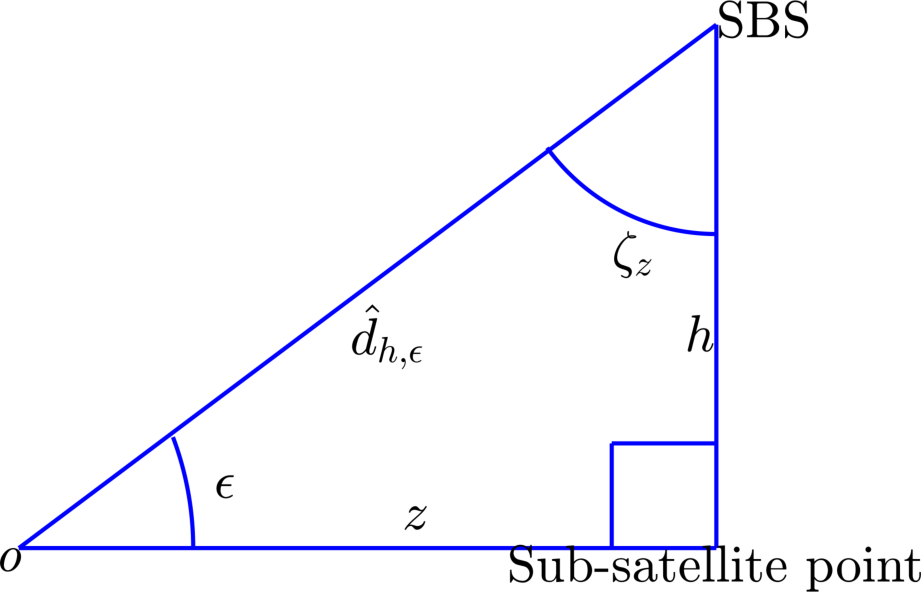
\includegraphics[width=0.7\linewidth]{triangle.pdf}
  \caption{Geometric interpretation of the variables in Appendix \ref{app:constantD} }
  \label{fig:triangle}
\end{figure}




\begin{remark}
  Not all all two-tier log-normal shadowing scenarios can be characterized and approximated with a one-tier manner with the distribution \eqref{eq:defexp}. For example $\upsilon_{}$ might be not within the region $0<\upsilon_{} \leq 1$. This can occur, for example, in case of significant differences in the LoS or NLoS variances in the shadowing, like is the case in the suburban/??? sceneario in the 3GPP specs. We could approximate separately the LoS and NLoS components by the exponential function, leading to two i.i.d. gamma processes of the LoS and NLoS component transmitter. Treating such two separate gamma process's (representing the aggregate STIR) of the two separate shadowing tiers can be challenging, and will be left out of the scope of this paper. Anyhow, the approach presented in the paper works for the urban scenario with the 3GPP specs, because the two-tier log-normal shadowing can be in a reasonable manner approximated by a one-tier shadowing model using a signle defective exponential distribution.
\end{remark}


\bibliographystyle{IEEEtran}
%\bibliography{IEEEabrv, bib}
\bibliography{IEEEabrv,source}


\end{document}
 
